\chapter{Analyse  Et Calcul  D’une Loi De Commande  Par Retour  D’état }
\addcontentsline{toc}{chapter}{Analyse  Et Calcul  D’une Loi De Commande  Par Retour  D’état }
 \section{Le modèle linéarisé est-il commandable?}
 
 
 
 
 
 
 \section{Calcule Des Valeurs Des Gains K et N Permettant De Remplir L’ensemble Des Conditions.}
 
\begin{center}
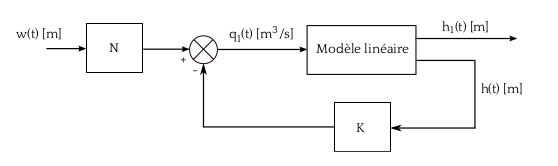
\includegraphics[scale=0.5]{fig2.png}
\captionof{figure}{\textit{ Retour d’état.}}
\label{fig2} 
\end{center}


